\chapter{Синтез $\mathcal{H}_2$-регулятора по состоянию}
\label{ch:chap2}
\section{Условие задачи}

\begin{itemize}
    \item Синтезировать соответствующий $\mathcal{H}_2$-регулятор вида $u = Kx$ по состоянию путем решения матричного уравнения Риккати.
    \item Найти передаточную функцию (матрицу) Ww→z(s) замкнутой системы от внешнего возмущения $w$ к регулируемому выходу $z$.
   \item Построить для $W_{w\rightarrow z}(s)$ графики покомпонентных АЧХ.
   \item Построить для $W_{w\rightarrow z}(s)$ график сингулярных чисел.
   \item Найти $\mathcal{H}_2$ и $\mathcal{H}_\infty$ нормы  $W_{w\rightarrow z}(s)$ .
   \item Задаться не менее, чем двумя вариантами гармонического внешнего возмущения
    w на основании полученных графиков АЧХ и сингулярных чисел $W_{w\rightarrow z}(s)$. 
    Среди выбранных возмущений должен присутствовать случай, близкий к «наихудшему» и ощутимо отличающийся от него по частоте.
    \item Для каждого из выбранных вариантов внешнего возмущения $w$ выполнить моделирование при нулевых начальных условиях
    на объекте управления и построить графики компонент регулируемого выхода $z(t)$.
    \item Сравнить полученные результаты для различных вариантов внешнего возмущения, сделать выводы.
\end{itemize}

\section{Решение задачи}

Найдём передаточную матрицу $W_{w\rightarrow z}(s)$ замкнутой системы в общем виде:

Уравнение системы состояния после замыкания и $z(t)$ с учётом регулятора:
$$
    \begin{cases}
        \dot{x} = (A+BK)x + B_w x \\
        z = (C_Z + D_Z K) x
    \end{cases}
$$
Возьмём преобразование Лапласа от обеих частей:
$$
    \begin{cases}
        sX = (A+BK)X + B_w X, \tab\rightarrow\tab X(s) = (sI - A - BK)^{-1} B_w W(s)\\
        Z(s) = (C_Z + D_Z K) X(s)
    \end{cases}
$$
Получаем:
$$
    Z(s) = (C_Z + D_Z K)(sI - A - BK)^{-1} B_w W(s)
$$
$$
    W_{w\rightarrow z}(s) = \frac{Z(s)}{W(s)} = (C_Z + D_Z K)*(sI - A - BK)^{-1} B_w
$$

Будем синтезировать $\mathcal{H}_2$-регулятор, решая \textbf{матричное уравнение Риккати}:
$$
    A^T Q + QA + C^T_Z C_Z - QB(D^T_Z D_Z)^{-1} B^T Q = 0, \tab K = -(D^T_Z D_Z)^{-1} B^T Q
$$

Если $C_Z^T D_Z = 0$, $D^T_Z D_Z$ - обратима, а также пары $(A, B_w)$ - стабилизируема, 
$(C_Z, A)$ - обнаруживаема, то существует решение $Q > 0$ уравнения Риккати, и соответствующий регулятор
делает замкнутую систему устойчивой и доставляет минимум ёё $\mathcal{H}_2$-норме.



\newpage
\subsection{Первый набор $(C_{Z1},D_{Z1})$}

Получим следующую матрицу регулятора: 
$$
    K = \begin{bmatrix}
        -0.5 & -1 
    \end{bmatrix}
$$
Получим следующую передаточную матрицу системы:
$$
    W_{w\rightarrow z}(s) = \begin{bmatrix}\frac{1}{s^{2} + 1s + 0.5} & \frac{-2s^{3} - 3s^{2} - 2s - 0.5}{s^{4} + 2s^{3} + 2s^{2} + 1s + 0.25} \end{bmatrix}^T
$$

 


Построим для $W_{w\rightarrow z}(s)$ графики покомпонентных АЧХ:
\begin{figure}[ht]
    \centering
    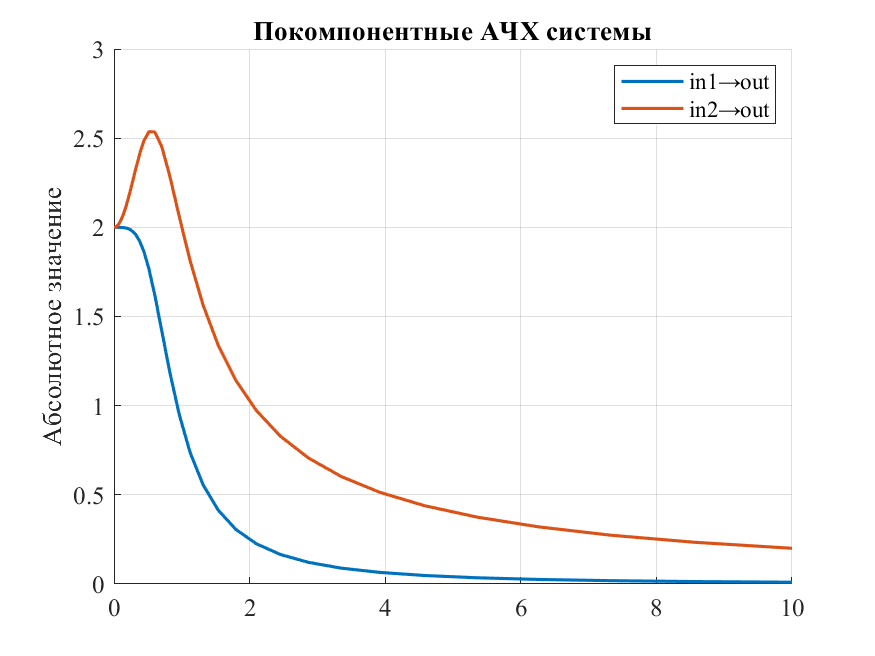
\includegraphics[width=0.8\textwidth]{freq_ampl_components1.png}
    \caption{Покомпонентные АЧХ}
  \end{figure}
Теперь построим для $W_{w\rightarrow z}(s)$ график сингулярных чисел:
\begin{figure}[ht]
  \centering
  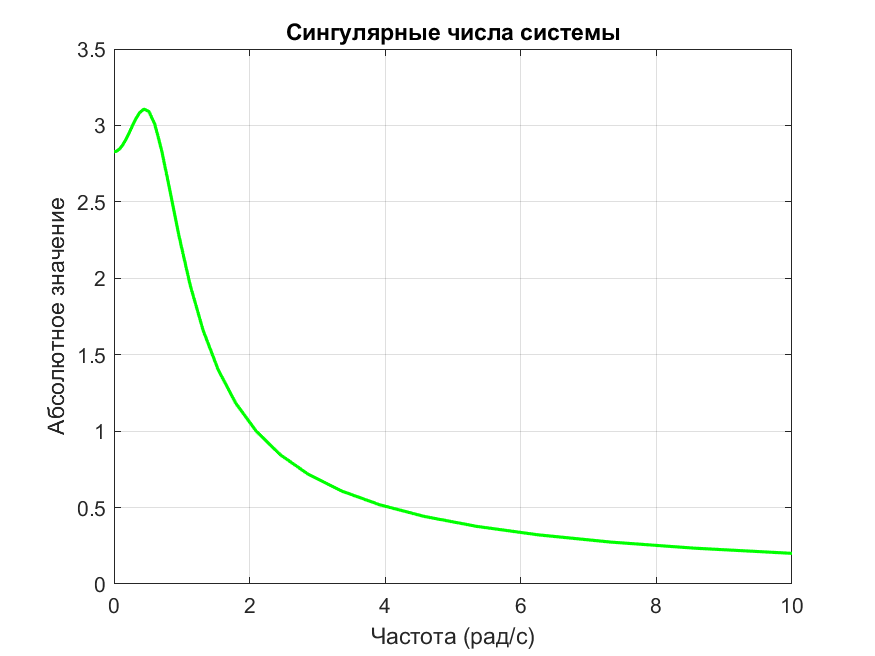
\includegraphics[width=0.8\textwidth]{singular_values1.png}
  \caption{Сингулярные числа}
\end{figure}
Нормы будем считать по следующим лекционным формулам, однако в \text{MATLAB} 
есть готовые реализации через функцию \text{norm}:
$$
    ||W||_{\mathcal{H}_2} = \bigg( \frac{1}{2\pi}\int_{-\infty}^{+\infty}trace(W^*(j\omega)W(j\omega))d\omega\bigg)^\frac{1}{2} \approx 2
$$

$$
    ||W||_{\mathcal{H}_\infty} = \sup_\omega \sigma_{max} (W(j\omega)) \approx 3.1
$$

На основании графиков АЧХ, выберем хорошую и плохую частоту $f_1, f_2$. 
Хорошей частотой для нас будет являться та, которая меньше увеличивает сигнал по амплитуде, и наоборот.
$$
    f_1 = 3 Hz, \tab f_2 = 0.55 Hz
$$

\newpage
\subsection{Первое гармоническое возмушение}
\begin{figure}[ht]
    \centering
    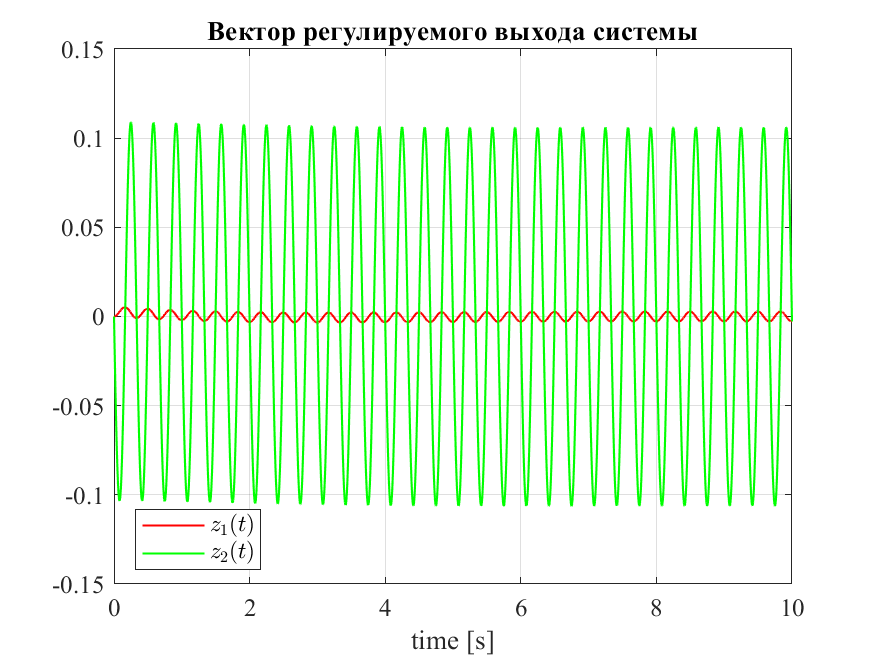
\includegraphics[width=0.8\textwidth]{z1.png}
    \caption{Моделирование -  регулируемый выход $z(t)$}
  \end{figure}
\newpage
\subsection{Второе гармоническое возмушение}
\begin{figure}[ht]
    \centering
    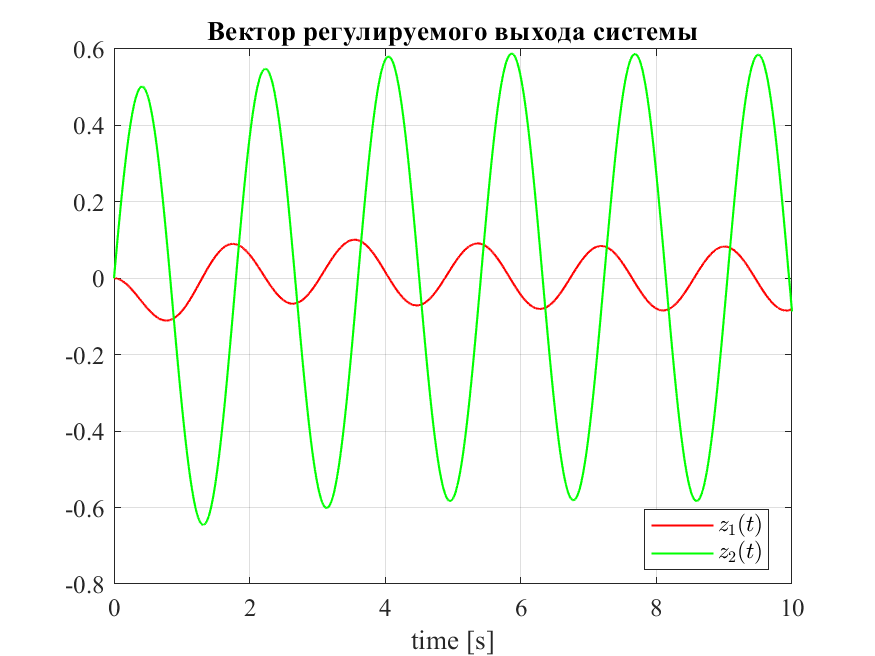
\includegraphics[width=0.8\textwidth]{z2.png}
    \caption{Моделирование -  регулируемый выход $z(t)$}
  \end{figure}

Как можно заметить, амплитуды возмущений в выходном сигнале $z(t)$ различаются по своему абсолютному значению, 
в плохом случае действительно сигнал увеличился почти в 4 раза больше по сравнению с "хорошей" частотой. 
$\mathcal{H}_2$-регулятор не решает задачу компенсации внешнего возмущения, и поэтому по итогу на 
выходе мы имеем некоторые колебания.

Также можно заметить, что пиковое сингулярное число системы действительно равняется $||W||_{\mathcal{H}_\infty}$.

\newpage
\subsection{Второй набор $(C_{Z2},D_{Z2})$}
Получим следующую матрицу регулятора: 
$$
    K = \begin{bmatrix}
        -0.5 &  -2.69
    \end{bmatrix}
$$
Получим следующую передаточную матрицу системы:
$$
    W_{w\rightarrow z}(s) = \begin{bmatrix}\frac{5s^{3} + 14.46s^{2} + 5.19s + 0.5}{s^{4} + 5.38s^{3} + 8.25s^{2} + 2.69s + 0.25}  & \frac{-5.38s^{3} - 15.5s^{2} - 5.38s - 0.5}{s^{4} + 5.38s^{3} + 8.25s^{2} + 2.69s + 0.25} \end{bmatrix}^T
$$



Построим для $W_{w\rightarrow z}(s)$ графики покомпонентных АЧХ:
\begin{figure}[ht]
    \centering
    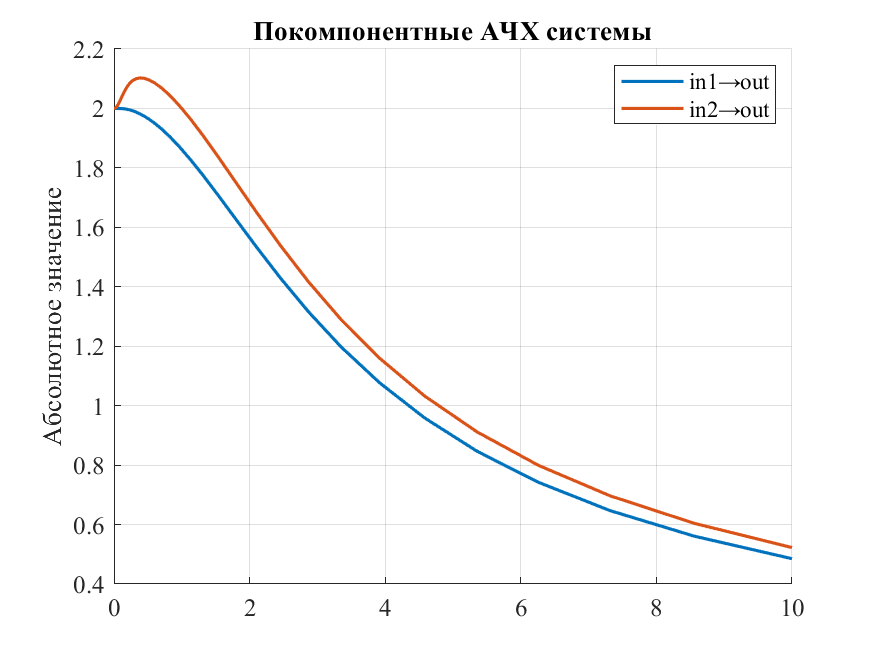
\includegraphics[width=0.8\textwidth]{freq_ampl_components2.png}
    \caption{Покомпонентные АЧХ}
  \end{figure}
Теперь построим для $W_{w\rightarrow z}(s)$ график сингулярных чисел:
\begin{figure}[ht]
  \centering
  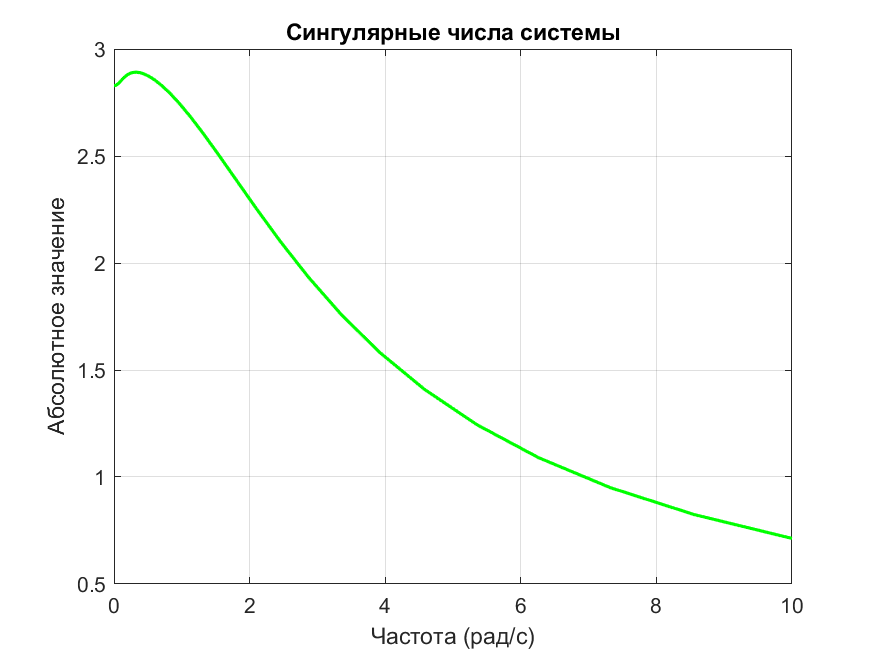
\includegraphics[width=0.8\textwidth]{singular_values2.png}
  \caption{Сингулярные числа}
\end{figure}
Нормы будем считать по следующим лекционным формулам, однако в \text{MATLAB} 
есть готовые реализации через функцию \text{norm}:
$$
    ||W||_{\mathcal{H}_2}   \approx 3.28
$$

$$
    ||W||_{\mathcal{H}_\infty}  \approx 2.89
$$

На основании графиков АЧХ, выберем хорошую и плохую частоту $f_1, f_2$. 
Хорошей частотой для нас будет являться та, которая меньше увеличивает сигнал по амплитуде, и наоборот.
$$
    f_1 = 10 Hz, \tab f_2 = 0.42 Hz
$$

\newpage
\subsection{Первое гармоническое возмушение}
\begin{figure}[ht]
    \centering
    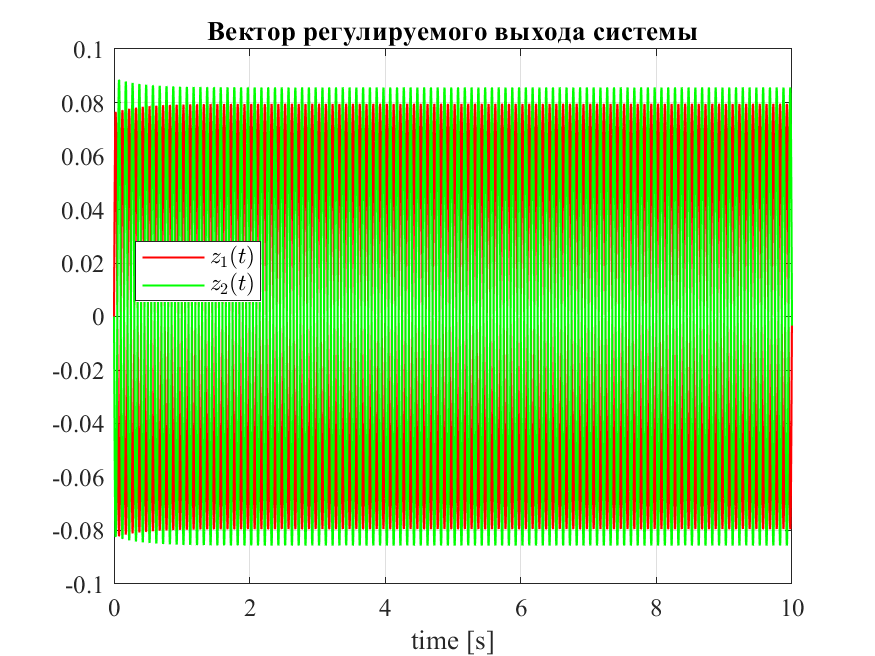
\includegraphics[width=0.8\textwidth]{z3.png}
    \caption{Моделирование -  регулируемый выход $z(t)$}
  \end{figure}
\newpage
\subsection{Второе гармоническое возмушение}
\begin{figure}[ht]
    \centering
    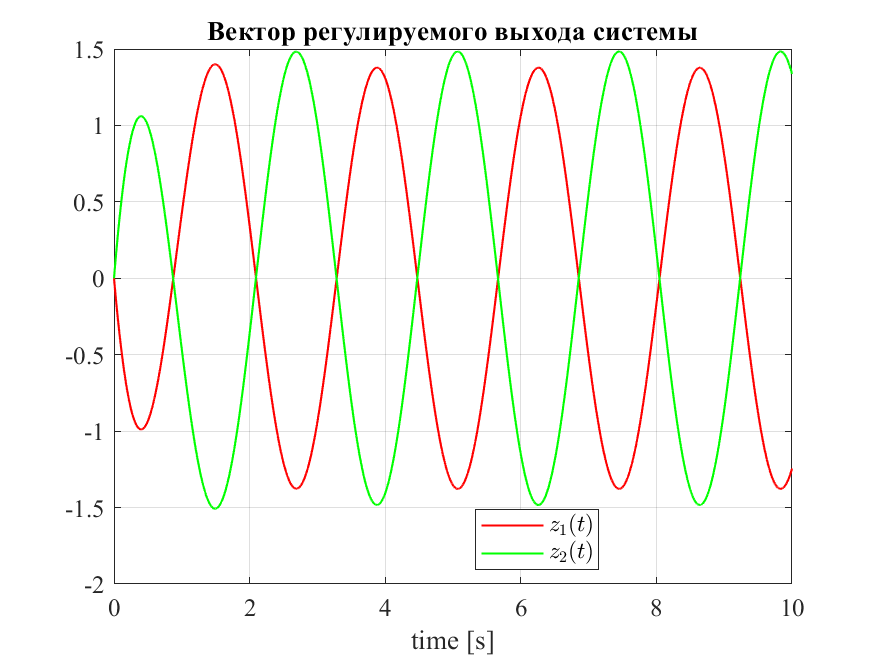
\includegraphics[width=0.8\textwidth]{z4.png}
    \caption{Моделирование -  регулируемый выход $z(t)$}
\end{figure}

Можно сделать аналогичные выводы, как и в первом наборе. Во втором возмущении сигнал приобрел нежелательную бОльшую амплитуду в связи с "неудачным" 
выбором частоты. Помимо этого, можно заметить, что выбор $(C_Z,D_Z)$ матриц регулируемого выхода не меняет общей картины, 
амплитуда возмущений при разных частота показывают одну и ту же тенденцию.

\subsection{Вывод}
В этом задании мы синтезировали $\mathcal{H}_2$-регулятор по состоянию 
и с помощью него убедились в справедливости воздейсвия АЧХ на амплитуду выходного сигнала регулируемого выхода $z(t)$, а также
независимости общей тенденции сигнала от выбора матриц $(C_Z,D_Z)$.
\endinput 